\documentclass[12pt]{report}
\usepackage{enumitem}        % enumeratie opties
\usepackage{color}           % extra kleuren
\usepackage[dutch]{babel}    % nederlandse sectieheaders i.p.v. engels
\usepackage[utf8]{inputenc}  % UTF-8 encoding
\usepackage{graphicx}        % laat toe om figuren (jpg, png, ...) te tonen
\usepackage[pdfpagelabels]{hyperref}        % hyperlinks in PDF
\usepackage[a4paper, margin=1.1in]{geometry}
\usepackage[toc,page]{appendix} %bijlage opties

\usepackage{usecases} % Voor use cases
\usepackage{float}

\hypersetup{pageanchor=false}

%VOORPAGINA
\title{Vakoverschrijdend Eindproject \\ Annotatietool\\Team 1\\ Eindverslag}
\author{ 
    Arnout Lenaerts                                       \\
    Bert De Saffel                                        \\
    Emiel Vandenbussche                                   \\
    Glenn Goossens                                        \\
    Nick van Hurck                                        \\
    Ruben Janssens                                        \\
    Timothy Thiecke                                       \\
    \vspace{0.2cm}                                        \\ 
    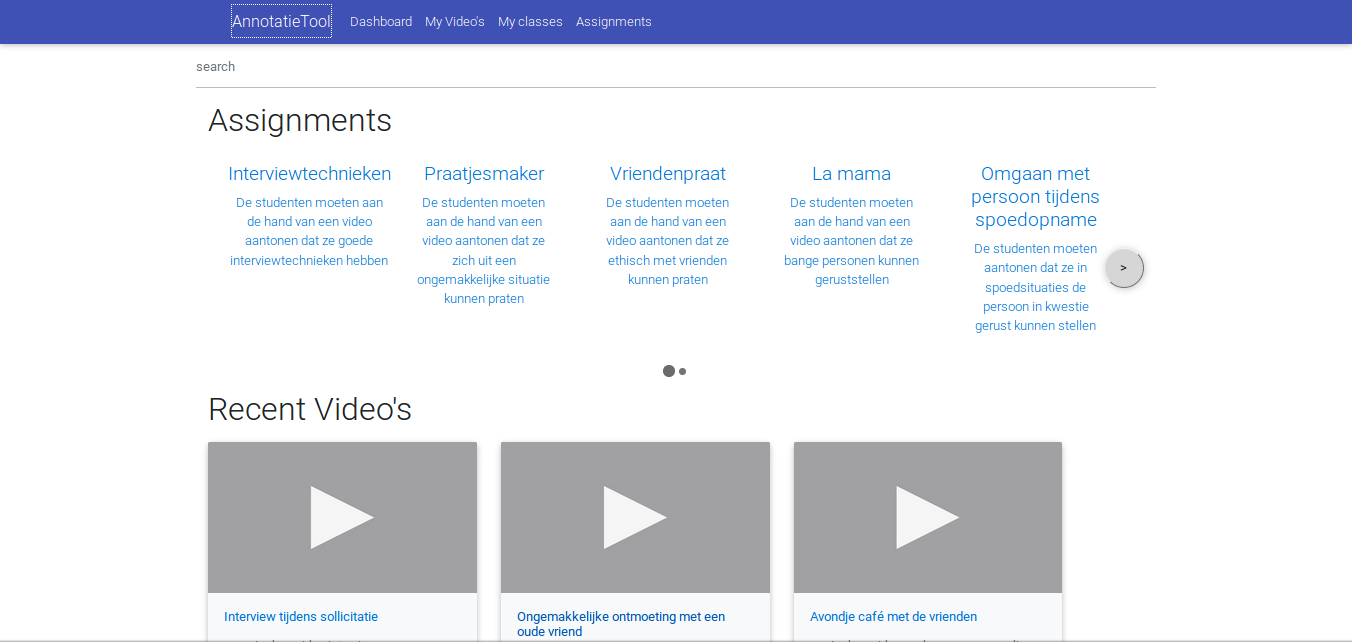
\includegraphics[width=0.9\textwidth]{titlepage}      \\
    Website: \url{http://annotatietool.tiwi.ugent.be/}
}
\date{\today}

%EIGEN MODIFICATIES
\setlength{\parindent}{0mm} % geen indendatie bij een nieuwe paragraaf
\graphicspath{{./img/}}     % figuren zijn te vinden in de img/ folder
\newcommand{\todo}[1]{
    {\color{red}\textunderscore{\textit{ToDo: #1}}}
}

\begin{document}
    \maketitle
    \tableofcontents
    \chapter{Inleiding}
\label{ch:inleiding}
\section{Context}
Binnen de UGent loopt een onderwijsinnovatie project waarin video annotatie wordt ingezet om communicatievaardigheden, die centraal staan in diverse opleidingsonderdelen in verschillende opleidingen, te trainen en op een authentieke manier te toetsen. Hiervoor wordt ingezet op peer-assessment, waarbij studenten elkaar feedback geven op gefilmde situaties waarin de student communicatievaardigheden toepast.
\section{Probleemstelling}
Er bestaat al commerci\"{e}le video-annotatiesoftware, maar deze hebben echter een duur prijskaartje en zijn bovendien complex om te gebruiken. Ondertussen heeft dit project wel een gratis alternatief gevonden, CommentBubble \footnote{\url{https://commentbubble.com/}}. CommentBubble maakt gebruik van YouTube om video's te hosten. Door het feit dat het videomateriaal enerzijds vertrouwelijke informatie bevat, en anderzijds om voldoende privacy te garanderen, gaat de voorkeur uit naar een annotatietool waarbij alle data intern opgeslagen word binnen de UGent.
\section{Doelstelling}
De video-annotatietool die ontworpen moet worden zal gebruikt worden door zowel docenten als studenten. Om installaties van de software te vermijden wordt er gekozen om deze tool te implementeren als een webapplicatie. 
\section{Overzicht van dit document}
In hoofdstuk \ref{ch:inleiding} werd de opdracht al toegelicht. In hoofdstuk \ref{ch:gebruikersaspecten} worden de noodzakelijke features besproken. In hoofdstuk \ref{ch:systeemarchitectuur} wordt de onderliggende structuur van het project besproken. In hoofdstuk \ref{ch:testplan} wordt besproken hoe het project uitgetest zal worden. In hoofdstuk \ref{ch:installatiehandleiding} wordt een overzicht gegeven hoe de software te installeren op een toestel.

    \chapter{Gebruikersaspecten}
\label{ch:gebruikersaspecten}
\section{High-Level requirements}
De applicatie kan gebruikt worden door twee type actoren. Een normale gebruiker (student) en een docent. De docent is een speciaal geval van een normale gebruiker met extra rechten, maar heeft ook dezelfde rechten als een normale gebruiker.
\subsection{Functionele requirements}
\subsubsection{Login}
\begin{itemize}
	\item De gebruiker kan zich inloggen via het UGent CAS-systeem of via een dummy systeem dat dit nabootst.
\end{itemize}
\subsubsection{Dashboard}
\begin{itemize}
	\item De gebruiker kan een video selecteren op het dashboard.
    \item De gebruiker kan een videobestand uploaden in de applicatie
 	\item De docent kan gebruikers koppelen aan een video.
 	\item De docent kan een deadline instellen van een video.
 	\item De docent kan een label toevoegen aan een video.
 	\item De docent kan groepjes van gebruikers aanmaken.
 	\item De docent kan de video's filteren per thema of categorie.
 	\item De docent kan quick comments beheren.
 	\item De docent kan quick comments koppelen aan een video.
 	\item De docent kan het niveau van toegankelijkheid voor de annotaties van een bepaalde video instellen.
	\item De docent kan voor een video of meerdere video's de annotaties exporteren.
 	\item De docent kan een .csv file uploaden.

\end{itemize}
\subsubsection{Video interactief}
\begin{itemize}
	\item De gebruiker kan op een specifiek moment een annotatie plaatsen.
	\item De gebruiker kan op een annotatie klikken om naar dat punt in de video te springen waarop de annotatie geplaatst is.
	\item De gebruiker kan een quick comment toevoegen op het huidige tijdstip van de video.
	\item De docent kan een video afspelen of pauzeren.
	\item De docent kan zoeken tussen alle annotaties van een bepaalde video.
\end{itemize}
\subsection{Niet-functionele requirements}
\begin{itemize}
 \item De website moet gebruiksvriendelijk zijn. De website moet eenvoudig te begrijpen zijn voor onervaren computergebruikers.
 \item Aangezien dat de video's vertrouwelijke inhoud kunnen bevatten, moet hiervoor de nodige beveiliging voorzien worden.
 \item Tijdens het typen van een annotatie zou de informatie voortdurend automatisch opgeslagen moeten worden zodat er geen werk verloren gaat. 
\end{itemize}

\subsection{Identificatie}
Gebruikers worden herkend aan de hand van hun UGent credentials. De applicatie kan alleen maar gebruikt worden door personen die verbonden zijn aan de UGent.

\section{Use case diagram}
Figuur 2.1 toont het use case diagram. Het systeem kent slechts 2 actoren: een normale gebruiker en een docent. Aangezien er een poging werd gedaan om het UGent CAS loginsysteem te gebruiken, bestaat er geen actie 'registreren'.
\begin{figure}
    \centering
        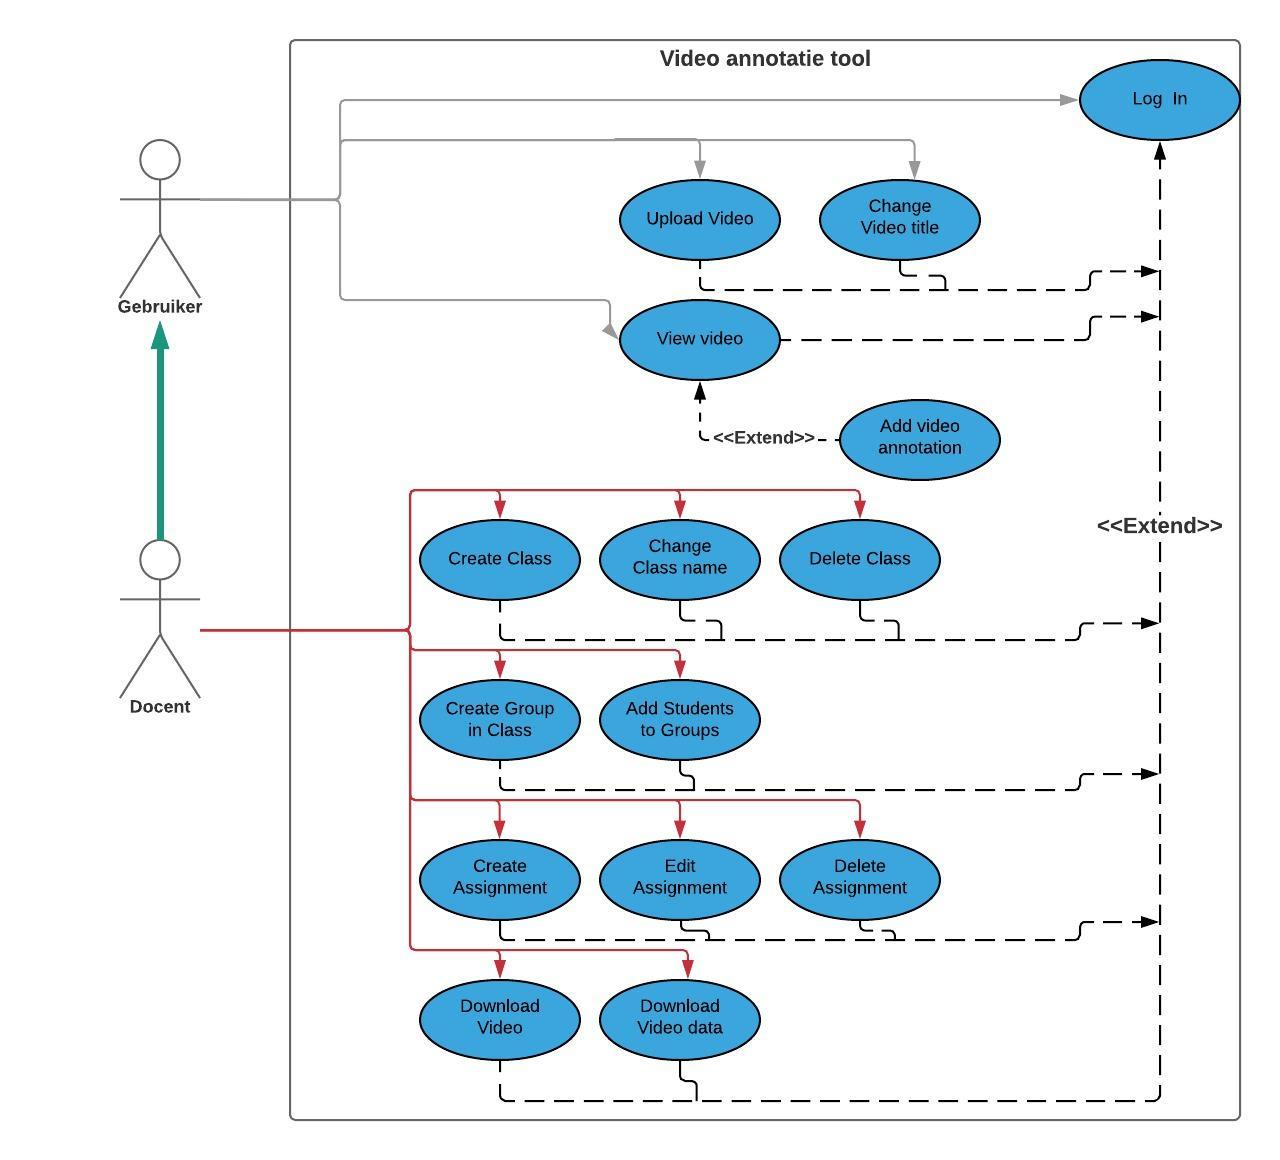
\includegraphics[width=\textwidth]{usecase2}
    \caption{Het use case diagram}
\end{figure}
\pagebreak
\section{Use cases}
\subsection{Upload video}
\begin{usecase}
	\addtitle{Use Case 1}{Upload video}
	\addfield{Actor:}{Gebruikers en docenten}
	\addfield{Trigger:}{De gebruiker selecteert de optie om een video te uploaden}
	\addscenario{Precondities:}{
		\item[-] De gebruiker is ingelogd (Log in use case)
		\item[-] Er is een opdracht aangemaakt door de docent (Create assignment use case)
	}
	\addscenario{Postcondities:}{
		\item[-] De video is geüpload en zichtbaar voor de gebruiker zelf en voor de gebruikers met wie de video gedeeld is
	}
	\addscenario{Basis flow:}{
		\item Het systeem toont het scherm waarop een video kan geüpload worden
		\item De gebruiker selecteert lokaal een video file
		\item Het systeem controleert of het om een video file gaat
		\item De gebruiker geeft de video een titel
		\item De gebruiker selecteert de bijhorende opdracht
		\item De gebruiker bevestigt de upload
		\item Het systeem slaat de video en bijhorende info op
		\item Het systeem toont de geüploade video
	}
	\addscenario{Alternatieve flow:}{
		\item[3a.] De gebruiker selecteerde een file dat geen video format is
		\begin{enumerate}
			\item[3a.1] Het systeem toont een foutboodschap en vraagt om de juist file te selecteren
			\item[3a.2] Terug naar stap 2
		\end{enumerate}      
	}
\end{usecase}
\pagebreak
\subsection{Add video annotation}
\begin{usecase}
	\addtitle{Use Case 2}{Add video annotation}
	\addfield{Actor:}{Gebruikers en docenten}
	\addfield{Trigger:}{De gebruiker selecteert een video}
	\addscenario{Precondities:}{
		\item[-] De gebruiker is ingelogd (Log in use case)
		\item[-] De gebruiker is een video aan het bekijken (View video use case)
	}
	\addscenario{Postcondities:}{
		\item[-] Een annotatie is opgeslagen voor een video
	}
	\addscenario{Basis flow:}{
		\item De gebruiker pauzeert de video stream
		\item De gebruiker geeft de tekst voor de annotatie in
		\item De gebruiker bevestigt de annotatie
		\item Het systeem slaat de annotatie met bijhorende timestamp op en geeft deze weer 
	}
	\addscenario{Alternatieve flow:}{
		\item[1a.] De video wordt niet gepauzeerd
		\begin{enumerate}
			\item[1a.1] De gebruiker selecteert een quick comment annotatie
			\item[1a.2.] Ga verder met stap 4
		\end{enumerate} 
		\item[2a.] Het gaat om een Drop down menu annotatie
		\begin{enumerate}
			\item[2a.1] De gebruiker selecteert de juist optie in de dropdown
			\item[2a.2] De gebruiker geeft bijhorende tekst in voor de annotatie
			\item[2a.3] Ga verder met stap 3
		\end{enumerate} 
	}
\end{usecase}
\pagebreak
\subsection{Create class}
\begin{usecase}
	\addtitle{Use Case 3}{Create class}
	\addfield{Actor:}{Docenten}
	\addfield{Trigger:}{De gebruiker selecteert de optie om een klas aan te maken}
	\addscenario{Precondities:}{
		\item[-] De gebruiker is ingelogd (Log in use case)
	}
	\addscenario{Postcondities:}{
		\item[-] Een nieuwe klas is aangemaakt met bijhorende gebruikers
	}
	\addscenario{Basis flow:}{
		\item Het systeem toont een pop-up waarin de gebruiker een klas kan aanmaken
		\item De gebruiker selecteert lokaal een .csv file met gebruikers
		\item Het systeem controleert of het een .csv file is en of deze correcte formattering gebruikt
		\item De gebruiker geeft de klas een naam
		\item De gebruiker bevestigt het aanmaken
		\item Het systeem slaat de klas en bijhorende gebruikers op
	}
	\addscenario{Alternatieve flow:}{
	        \item [3a.] Het .csv bestand heeft geen geldig formaat
	        \begin{enumerate}
	         \item [3a.1] Het systeem toont een gepaste melding
	         \item [3a.2] Keer terug naar stap 2
	        \end{enumerate}

	
	
	}
\end{usecase}
\pagebreak
\subsection{Create assignment}
\begin{usecase}
	\addtitle{Use Case 6}{Create assignment}
	\addfield{Actor:}{Docenten}
	\addfield{Trigger:}{De gebruiker selecteert de optie om een opdracht aan te maken
	}
	\addscenario{Precondities:}{
		\item[-] De gebruiker is ingelogd (Log in use case)
	}
	\addscenario{Postcondities:}{
		\item[-] Een nieuwe opdracht is aangemaakt
	}
	\addscenario{Basis flow:}{
		\item Het systeem toont een pop-up waarin de gebruiker een opdracht kan aanmaken
		\item De gebruiker geeft de opdracht een naam
		\item De gebruiker activeert de gewenste annotaties en vult de juiste bijhorende waarden in
		\item De gebruiker geeft aan of de annotaties privé zijn of niet
		\item De gebruiker selecteert voor welke klas of groep de opdracht is
		\item De gebruiker geeft aan wie de uploads mag doen (docent of gebruiker)
		\item De gebruiker geeft mogelijk een deadline mee
		\item Het systeem controleert de data
		\item Het systeem maakt de opdracht aan en slaat de data op
		\item Het systeem toont een overzicht van alle opdrachten
	}
	\addscenario{Alternatieve flow:}{
		\item[8a.] De data is niet volledig
		\begin{enumerate}
			\item[8a.1] Het systeem toont een foutboodschap
			\item[8a.2] De gebruiker overloopt opnieuw vanaf stap 2
		\end{enumerate} 
	}
\end{usecase}
\pagebreak
\subsection{Download video data}
\begin{usecase}
	\addtitle{Use Case 8}{Download video data}
	\addfield{Actor:}{Docenten}
	\addfield{Trigger:}{De gebruiker selecteert de optie om de video data te downloaden
	}
	\addscenario{Precondities:}{
		\item[-] De gebruiker is ingelogd (Log in use case)
		\item[-] De gebruiker is een video aan het bekijken (View video use case)
	}
	\addscenario{Postcondities:}{
		\item[-] De gebruiker heeft een lokale versie van de verschillende annotaties van de video	
	}
	\addscenario{Basis flow:}{
		\item Het systeem pauzeert de video
		\item Het systeem vraagt of de gebruiker zeker is
		\item De gebruiker bevestigt
		\item Het systeem genereert de data file
		\item Het systeem start een download van die file naar de computer van de gebruiker
	}
	\addfield{Alternatieve flow:}{/
	}
\end{usecase}
\pagebreak




\section{Backlog}
De volgende lijst stelt de product backlog voor, inclusief volgende attributen: extra uitleg, de prioriteit, de complexiteit, in welk sprint deze feature afgewerkt is en eventueel extra opmerkingen.

\begin{itemize}
\setlength\itemsep{2em}
 \item Als een gebruiker wil ik een video kunnen uploaden (\textbf{Sprint 1})
        
        \textbf{Uitleg} Het uploaden van een video is \'e\'en van de basisfunctionaliteiten.
        
        \textbf{Prioriteit}: 5/5  \textbf{Complexiteit}: 3/5
        
 \item Als een gebruiker wil ik een video kunnen bekijken (\textbf{Sprint 1})

        \textbf{Uitleg}: Het bekijken van een video is \'e\'en van de basisfunctionaliteiten.

        \textbf{Prioriteit}: 5/5 \textbf{Complexiteit}: 2/5
        
 \item Als een gebruiker wil ik annotaties kunnen plaatsen op een video (\textbf{Sprint 2})

        \textbf{Uitleg}: Het toevoegen van annotaties is \'e\'en van de basisfunctionaliteiten.

        \textbf{Prioriteit}: 5/5 \textbf{Complexiteit}: 3/5
 \item Als een gebruiker wil ik quick annotations toevoegen aan een video (\textbf{Sprint 2})
        
        \textbf{Uitleg}: Het toevoegen van quick annotations is een uitbreiding op de normale annotaties.
            \textbf{Prioriteit}: 4/5 \textbf{Complexiteit}: 1/5

            
 \item  Als een gebruiker wil ik naar een punt in de video springen waar een annotatie staat zodat ik de annotatie kan bekijken (\textbf{Sprint 2})

        \textbf{Uitleg}: Een gebruiker wil een eenvoudige manier om het filmpje af te spelen op de plaats waar een annotatie geplaatst is

        \textbf{Prioriteit}: 3/5 \textbf{Complexiteit}: 1/5
 \item Als een gebruiker wil ik een dashboard zodat ik een overzicht heb van mijn taken en video's (\textbf{Sprint 2})

        \textbf{Uitleg}: Het dashboard is de eerste pagina dat getoond wordt wanneer een gebruiker inlogt. Deze pagina moet direct een overzicht bieden van de nog te maken taken, en video's die kunnen bekeken worden

        \textbf{Prioriteit}: 4/5 \textbf{Complexiteit}: 3/5
 \item Als een docent wil ik klasgroepen importeren uit een .csv bestand zodat ik een overzicht heb van mijn studenten (\textbf{Sprint 2})

        \textbf{Uitleg}: Aangezien het UGent CAS systeem uiteindelijk niet op de applicatie is aangesloten, kunnen de klasgroepen niet rechtstreeks vanuit dit systeem gehaald worden. De applicatie laat toe een .csv bestand up te loaden die een .csv export van Minerva nabootst zodat hieruit klasgroepen kunnen gemaakt worden.

        \textbf{Prioriteit}: 3/5 \textbf{Complexiteit}: 4/5
 \item  Als een gebruiker wil ik taken bekijken zodat ik daar een video voor kan uploaden (\textbf{Sprint 3})
        
        \textbf{Uitleg}: De gebruiker moet een overzicht hebben van zijn taken om te weten waar hij een video kan uploaden
        
        \textbf{Prioriteit}: 3/5 \textbf{Complexiteit}: 3/5
 \item Als een gebruiker wil ik kunnen inloggen zodat ik gebruik kan maken van de applicatie (\textbf{Sprint 3})

        \textbf{Uitleg}: Een geldig UGent email-adres hebben is verplicht om gebruik te kunnen maken van de applicatie. Indien de gebruiker een geldig UGent email-adres heeft kan de gebruiker inloggen op de applicatie.


        \textbf{Prioriteit}: 5/5 \textbf{Complexiteit}: 4/5

        \textbf{Opmerking}: Deze feature werd ook al eens in sprint 1 opgenomen, maar er was onvoldoende kennis over het UGent Cas systeem om de implementatie te starten

        
        
\end{itemize}



    \chapter{Systeemarchitectuur}
\label{ch:systeemarchitectuur}
\section{High-level systeem model}
Het project bestaat uit twee delen. Het eerste deel is de webapplicatie die gebruikt wordt door de actor. Het tweede deel is de MP4 Converter. Dit is een aparte module dat video's van allerlei formaten omvormt tot het standaardformaat dat gebruikt wordt in de applicatie, namelijk .mp4.
\subsection{Webapplicatie}
De webapplicatie wordt geprogrammeerd met gebruik van de MEAN \footnote{\url{http://mean.io/}} stack. Dit is een verzameling van technologieën die samen gebruikt worden om webapplicaties te ontwikkelen. De MEAN stack bevat volgende onderdelen:
\begin{itemize}
 \item \textbf{M}ongoDb: Dit is een open source NoSQL databank dat gebruik maakt van JSON documenten om gegevens te bewaren. 
 \item \textbf{E}xpress: Dit is een implementatie van Node dat geschikt is voor het opstellen van webservers. 
 \item \textbf{A}ngular: Dit is een client-side javascript framework dat geschikt is voor het creëren van dynamische webapplicaties. De interactie tussen het DOM en javascript wordt vereenvoudigt met Angular.
 \item \textbf{N}ode.js: Dit is een javascript runtime omgeving met als onderliggende basis de javascript engine van Chrome. Een gevolg van Node is het node packaging systeem (npm) dat toelaat om modules toe te voegen aan een applicatie met slechts één lijn code.
\end{itemize}
Hoe deze componenten met elkaar samenwerken kan bekeken worden op figuur \ref{fig:deploymentdiagram}.

\subsection{MP4 Converter}
De MP4 Converter is geprogrammeerd in Java en wordt gebruikt door de webapplicatie om videobestanden van verschillende formaten om te zetten naar het mp4 formaat. Als onderliggende basis wordt gebruik gemaakt van \texttt{ffmpeg} \footnote{\url{https://ffmpeg.org/}}. Dit is een handige tool dat toelaat om video's of geluid op te nemen en te converteren. Deze applicatie maakt enkel gebruik van het converteren van een video. De MP4 Converter is met andere woorden een Java wrapper voor ffmpeg met slechts beperkte functionaliteit.




\section{Klassendiagram}
\begin{figure}[ht]
	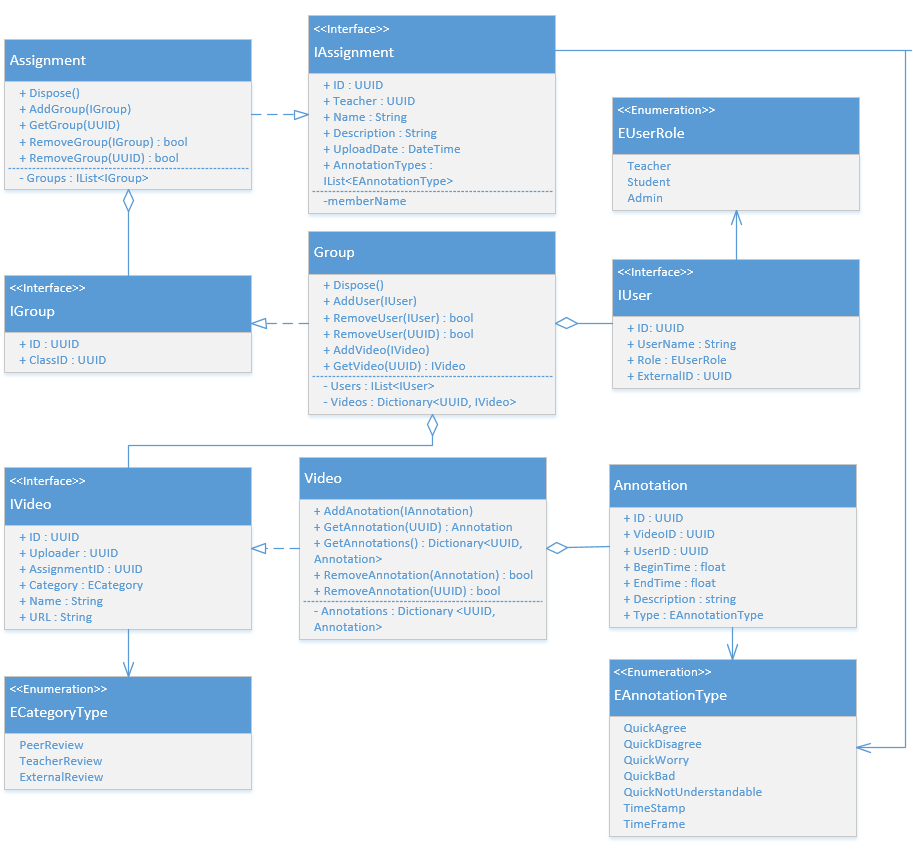
\includegraphics[width=\textwidth]{klassendiagram}
	\caption{Het klassendiagram}
	\label{fig:klassendiagram}
\end{figure}

In figuur \ref{fig:klassendiagram} is een overzicht te vinden van het klassendiagram. Dit diagram komt overeen met de implementaties van de verschillende database modelklassen en de manier hoe ze in relatie tot elkaar staan in de backend.
%% TODO: Informatie uitbreiden

\section{Deploymentdiagram}
\begin{figure}[ht]
	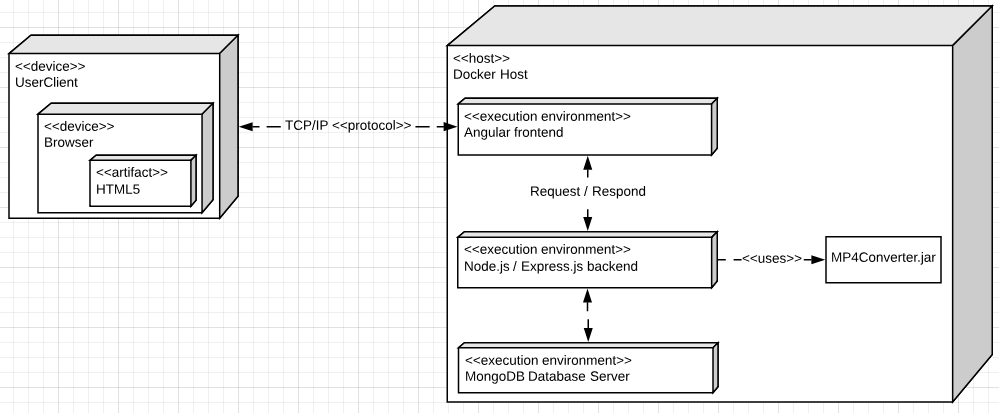
\includegraphics[width=\textwidth]{deploymentdiagram}
	\caption{Het deploymentdiagram}
	\label{fig:deploymentdiagram}
\end{figure}
In figuur \ref{fig:deploymentdiagram} is een overzicht te vinden van het deploymentdiagram. De applicatie draait in drie aparte docker containers op de server: de Node.js container (backend), de Angular frontend container en de MongoDB database container. 

\section{Databank}
De databank is opgesteld in MongoDB. Dit is een NoSQL omgeving waardoor het moeilijk is om een databankdiagram op te stellen. Om een overzicht te hebben van de relaties tussen de verschillende klassen zoals ze zijn ge\"implementeerd in de code kan gekeken worden naar het klassendiagram op figuur \ref{fig:klassendiagram}


\section{Sequentiediagrammen}

\begin{figure}
	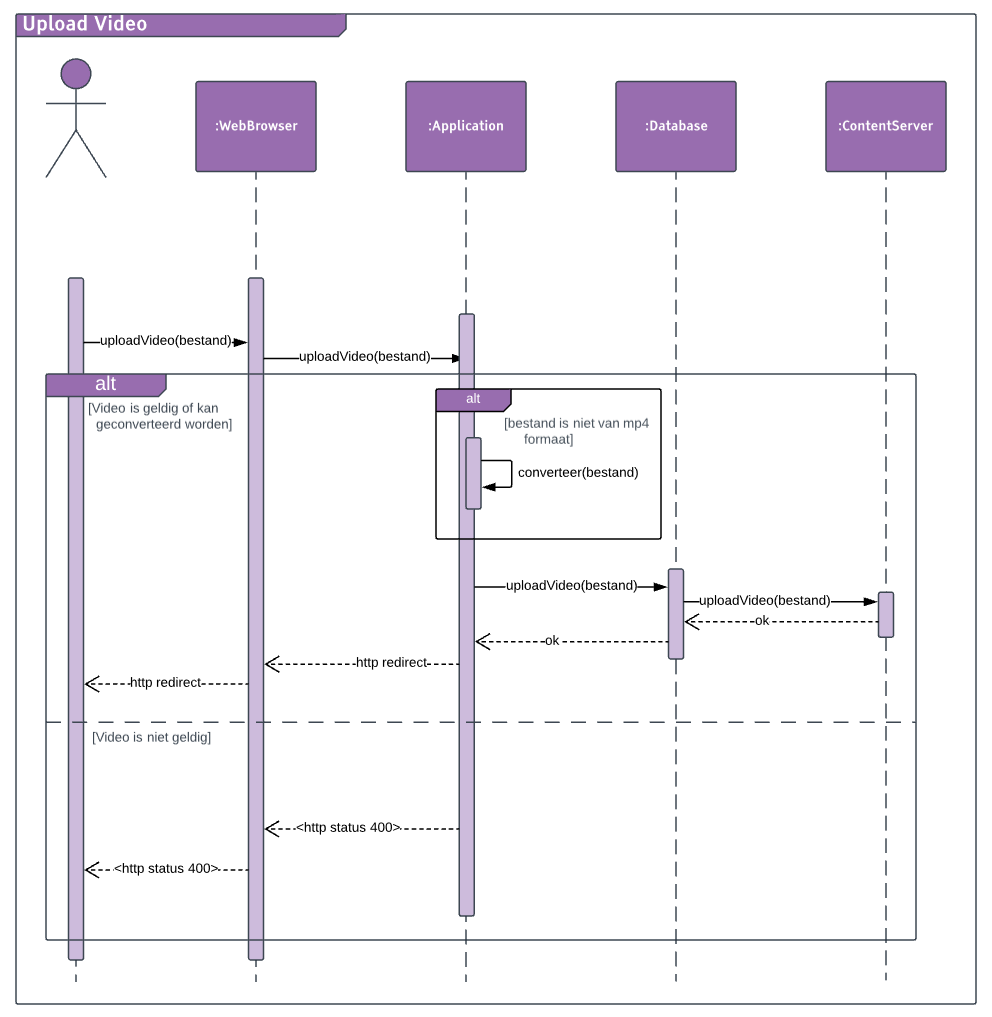
\includegraphics[width=\textwidth]{seq_diagram//SEQ_Upload_Video}
	\caption{Sequentiediagram van upload video}
	\label{fig:seq_upload_video}
\end{figure}

\begin{figure}
	\includegraphics[width=\textwidth]{seq_diagram//SEQ_plaats_annotatie}
	\caption{Sequentiediagram van show video}
	\label{fig:seq_show_video}
\end{figure}
Figuren \ref{fig:seq_upload_video} en \ref{fig:seq_show_video} zijn sequentiediagrammen van twee belangrijke events die kunnen voorkomen in de applicatie. De verschillende events maken gebruik van synchrone gebruikersinput die asynchroon wordt behandeld.

    %% TESTPLAN
\chapter{Testplan}
\label{ch:testplan}
De applicatie wordt op twee verschillende manieren getest om fouten of onduidelijkheden te voorkomen. De volgende onderdelen bespreken de verschillende soorten testen en wanneer deze uitgevoerd worden.

\section{Unit testen}
Unit testen dienen om specifieke functionaliteiten van modules te testen zonder afhankelijk te zijn van andere implementaties door gebruik te maken van mock-objecten. Zulke objecten kunnen bijvoorbeeld de database of langdurige operaties vervangen. 
\newline

Dit project heeft twee soorten unit testen. Er bestaan unit testen voor zowel de webapplicatie als het Java-stuk.

De unit-testen zijn geschreven met Jasmine. Meer specifiek de node versie hiervan, \texttt{jasmine-node}. Voor volgende functionaliteiten zijn er testen geschreven:
\begin{itemize}
 \item Inloggen op de applicatie
 \item Plaatsen van annotaties
 \item Aanmaken van groepen op basis van een .csv bestand
\end{itemize}


Aangezien een videobestand meerdere formaten kan aannemen, zijn er ook unit testen die de conversie van zo een bestand test. In de applicatie zijn enkel .mp4 bestanden toegelaten.
\newline

\subsection{Testsuite Webapplicatie}
De volgende scenario's worden getest op de webapplicatie.
\subsubsection{Met betrekking tot het plaatsen van annotaties}
\begin{itemize}
 \item Er wordt een annotatie aan een video toegevoegd indien de annotatie geldig is.
 \item Er wordt een fout gegeven wanneer een annotatie ongeldig is. Een annotatie is ongeldig wanneer: 
    \begin{enumerate}
      \item de begintijd een negatieve waarde bevat.
      \item wanneer de eindtijd eerder dan de begintijd komt.
    \end{enumerate}
\end{itemize}
\subsubsection{Met betrekking tot het inloggen in de applicatie}
\begin{itemize}
 \item De gebruiker kan inloggen indien een correct UGent email-adres en paswoord gebruikt wordt.
 \item Er wordt een fout gegeven indien een paswoord of een gebruikersnaam incorrect is.
\end{itemize}

\subsubsection{Met betrekking tot het aanmaken van groepen}
 \begin{itemize}
  \item Er wordt een klasgroep aangemaakt indien een correct .csv bestand meegegeven wordt. Een correct .csv bestand heeft het volgende formaat:
  
  \texttt{Offici\"ele code;Voornaam;Familienaam;UGent-email;Rol;Subgroep}
 \end{itemize}



\subsection{Testsuite MP4 converter}
De volgende scenario's worden getest op de MP4 converter.
\begin{itemize}
 \item Er wordt een correcte conversie van een toegelaten videobestand naar MP4 formaat uitgevoerd.
 \item Er wordt een fout weergegeven indien een bestand geen extensie heeft.
 \item Er wordt een fout gegeven indien een bestand een niet toegelaten extensie heeft.
 \item Er wordt een fout gegeven indien het bestand niet bestaat
\end{itemize}


Omdat de broncode nodig is om de testen uit te voeren en aangezien dit pas besproken wordt in \ref{sec:download_repository} hoe dit moet gebeuren, wordt pas in sectie \ref{sec:test_exec} besproken hoe de testen kunnen uitgevoerd worden.



\section{Usability testen}
Uiteindelijk moet de applicatie bruikbaar zijn voor personen die het zullen gebruiken. Er wordt aan het einde van een sprint aan een onafhankelijke persoon gevraagd om de functionaliteiten die ge\"implementeerd zijn te testen. Wanneer er onduidelijkheden zijn wordt er samen met deze persoon naar een alternatief gezocht. Er wordt een kort verslag gemaakt  met commentaar van de gebruiker.

\subsection{Reflectieverslag Usability test sprint 2}
De webapplicatie die online staat na sprint 2 heeft volgende beperkte functionaliteiten:
\begin{itemize}
\item Overzicht van video's en assignments
\item Video uploaden
\item Video bekijken
\item Annotatie plaatsen
\item Groepen bekijken
\item Assignments bekijken
\end{itemize}

Testpersonen, Yana De Brouwer, Herman Goossens \& Marijke Van Wayenberg, hebben deze functionaliteiten uitgetest zonder veel extra uitleg en op basis van de test-sessie enkele bevindingen aangebracht.
\begin{itemize}
\item Het is niet duidelijk bij het dashboard of de assignments en video's voor jou bedoelt zijn.
\item Een video afspelen werkt zoals het zou moeten en is makkelijk te bereiken vanuit het dashboard.
\item Er is geen melding of een video uploaden al dan niet gelukt of bezig is. Je wordt gewoon herleid naar de hoofdpagina.
\item Het overzicht van de assignments is bombastisch en dus niet overzichtelijk, idem groups.
\item De styling van de applicatie kan beter.
\end{itemize}

Deze bevindingen worden meegenomen naar de laatste sprint en worden gebruikt om verbeteringen aan te brengen in de applicatie.

    %% INSTALLATIEHANDLEIDING
\chapter{Installatiehandleiding}
\label{ch:installatiehandleiding}
Dit hoofdstuk bespreekt hoe het software-pakket lokaal op een toestel kan 
draaien. De volgende logingegevens kunnen gebruikt worden om te authenticeren op de applicatie:

\begin{table}[ht]
 \centering
 \begin{tabular}{l | l | l}
    username & passwoord & rol \\
    \hline
    docent & test & docent \\
    student & test & student
 \end{tabular}
\end{table}





\section{Hardware en Software}
\label{sec:hardware_and_software}
De applicatie kan op volgende besturingssystemen draaien:
\begin{itemize}
	\item Linux (32 en 64 bit)
	\item macOS (64 bit)
	\item Windows 7 of hoger (32 en 64 bit)
\end{itemize}

Verder moeten ook nog volgende softwarepakketten ge\"installeerd worden.
\begin{itemize}
\item Node.js (minimum v8.9.4): \url{https://nodejs.org/en/download/}. Opteer voor het 
\textit{.msi} bestand voor Windows en het .pkg bestand voor macOS zoals te zien op figuur \ref{fig:node_1} om de installatieprocedure zo eenvoudig 
mogelijk uit te voeren. Controleer of dit juist ge\"installeerd is door het commando \texttt{node -v} uit te voeren in een terminal of console.
\begin{figure}[ht]
        \centering
 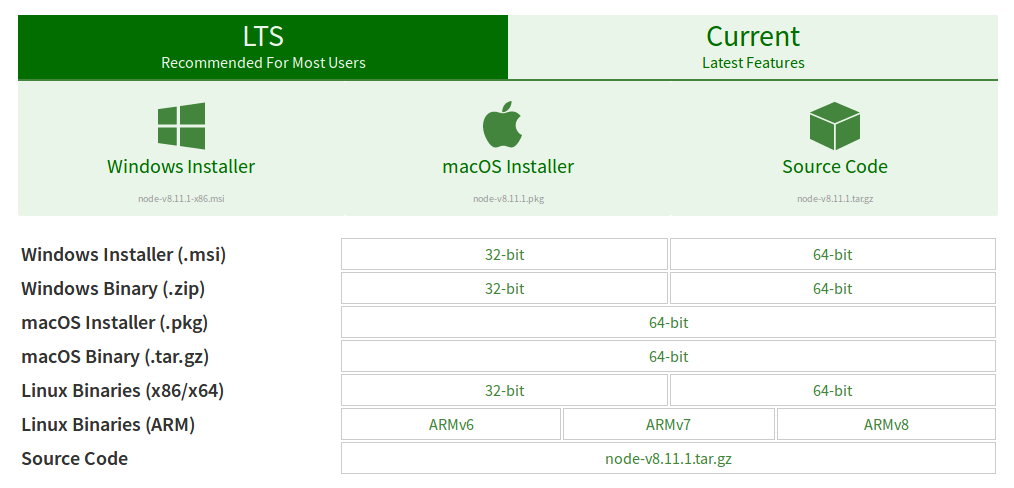
\includegraphics[width=0.9\textwidth]{install_guide/node_1}
 \caption{Node pagina - download}
 \label{fig:node_1}

\end{figure}
\item MongoDB (minimum v2.6.10): \url{https://www.mongodb.com/download-center} 
en klik op \texttt{Community Server} zoals aangegeven in figuur \ref{fig:mongo_1}.
\begin{figure}[ht]
\centering
 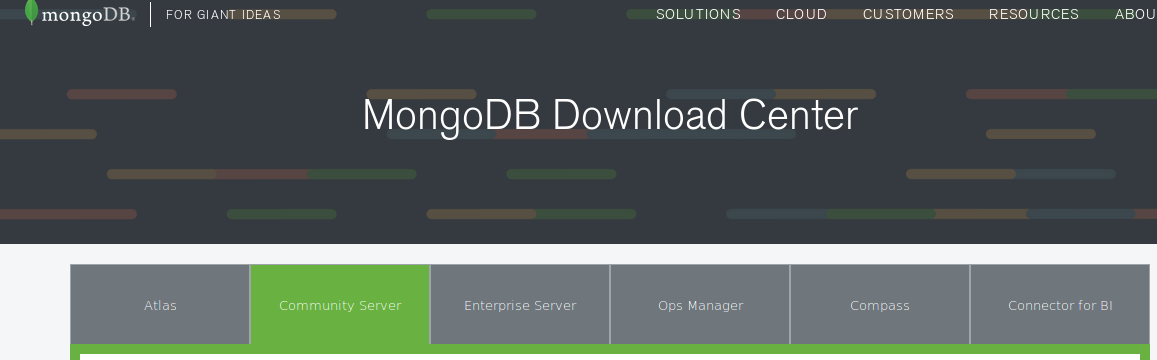
\includegraphics[width=0.9\textwidth]{install_guide/mongo_1}
 \caption{Mongo pagina - Community Server}
 \label{fig:mongo_1}
\end{figure}
Klik vervolgens op het gewenste besturingssysteem en klik dan op download zoals te zien op figuur \ref{fig:mongo_2}. Controleer of dit juist ge\"installeerd is door het commando \texttt{mongo  --version} uit te voeren in een terminal of console.
\begin{figure}[ht]
\centering
 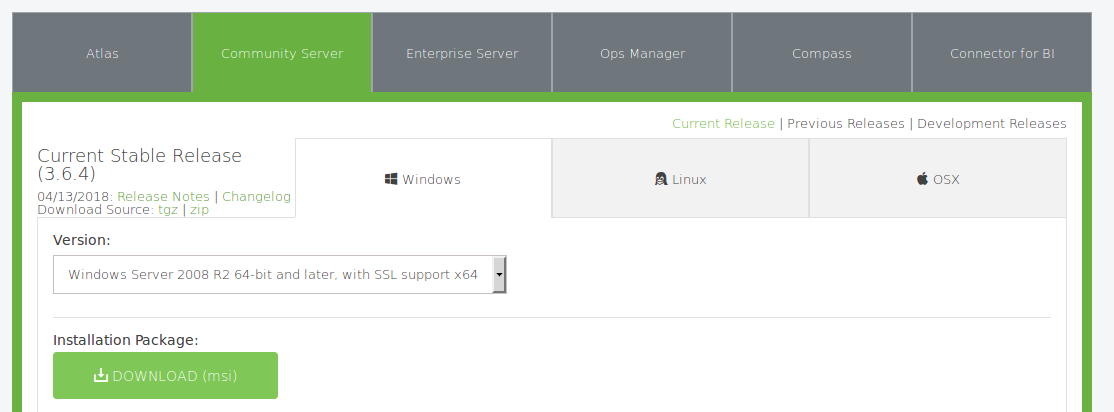
\includegraphics[width=0.9\textwidth]{install_guide/mongo_2}
 \caption{Mongo pagina - download}
 \label{fig:mongo_2}
\end{figure}

    \item Java 8 (minimum $JDK\;8u171$): \url{https://www.java.com/en/download/win10.jsp} : Klik op de download knop en volg de installatieprocedure. Controleer of dit juist ge\"installeerd is door het commando \texttt{java --version} uit te voeren in een terminal of console.
    
    \item ffmpeg : Dit bevat enkel builds voor Windows en macOS. Een .bz2 bestand kan teruggevonden worden op \url{https://ffmpeg.org/download.html}. Om te controleren of dit programma correct is geïnstalleerd kan het commando \texttt{ffmpeg} uitgevoerd worden in de console of terminal.

\end{itemize}

\section{Downloaden repository}
\label{sec:download_repository}
Nadat al de benodigde software ge\"installeerd is moet de broncode op het toestel geplaatst worden. Dit kan op twee manieren:
\begin{enumerate}
    \item Indien \textit{git} ge\"installeerd is op het toestal kan het commando 
    
    \texttt{git clone https://github.ugent.be/bp-vop-2018/annotatietool-01.git} 
    
    gebruikt worden. Dit zal een folder aanmaken met de naam \texttt{annotatietool-01} waarin de broncode terug te vinden is.
    
    \item Indien het toestel geen \textit{git}  heeft, kan de repository nog altijd manueel gedownload worden via \url{https://github.ugent.be/bp-vop-2018/annotatietool-01}. Klik op 
\texttt{Clone or download} en dan \texttt{Download ZIP} zoals te zien op figuur \ref{fig:git_1}. Dit zal een ZIP 
bestand downloaden waarin de broncode terug te vinden is. Plaats de inhoud van het ZIP bestand (folder genaamd \texttt{annotatietool-01}) op het toestel.
\begin{figure}[ht]
 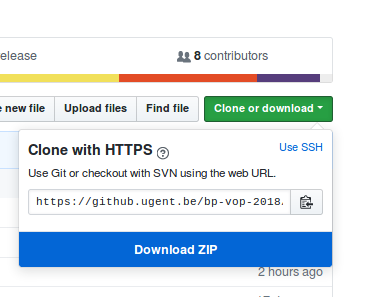
\includegraphics[width=0.5\textwidth]{install_guide/git_1}
 \centering
 \caption{Github pagina : download}
 \label{fig:git_1}
\end{figure}
\end{enumerate}

\subsection{Structuur repository}
Al de broncode van het project bevindt zich in \texttt{annotatietool-01}. De belangrijkste items in deze folder zijn:
\begin{itemize}
 \item \textbf{app.js} : Dit bestand is het startpunt van de applicatie.
 \item \textbf{src}    : Deze folder bevat alle code in verband met de frontend.
 \item \textbf{backend} : Deze folder bevat all code met betrekking tot de backend.
 \item \textbf{spec}    : Deze folder bevat integratietesten voor de webapplicatie (zie \ref{sec:test_exec_web} om de testen uit te voeren).
 \item \textbf{java}    : Deze folder bevat het java-gedeelte van het project (de MP4 converter). De unit testen zitten ook in deze folder (zie \ref{sec:test_exec_java} om de testen uit te voeren).
\end{itemize}




\section{Runnen applicatie}
\label{sec:run_app}
Er bestaan twee mogelijkheden om de applicatie te draaien op een lokaal toestel. 
\subsubsection{Docker}
Hiervoor moet Docker ge\"installeerd worden op het toestel. Navigeer naar \url{https://store.docker.com/search?type=edition&offering=community} om naar een lijst te gaan van de community edition van Docker per besturingssysteem. Kies de versie dat past bij het besturingssysteem van het toestel en voer de installatieprocedure uit.

Indien Docker ge\"installeerd is op het toestel kan het commando \texttt{./buildandrun.sh} uitgevoerd worden in de root directory van het project (annotatietool-01).
Als de docker frontend container in productie gedeployed wordt, dan moet de \texttt{ --disable-host-check} flag verwijdert worden uit de Dockerfile, alsook moet de host gespecifieerd worden voor de productieomgeving.
De webapplicatie kan vanaf nu bediend worden op het lokaal adres \texttt{localhost:9000} via een webbrowser.
\subsubsection{Zonder docker}
Indien geen gebruik gemaakt wordt van docker moet de technologiestack 
zelfstandig ge\"installeerd worden. Voer volgende stappen uit.
\begin{enumerate}
	\item Navigeer naar de \texttt{project} folder (annotatie-tool-01/project).
	\item Open een terminal of de console (afhankelijk van het besturingssysteem) 
	      en voer het commando \texttt{npm install} uit. Dit zal alle nodige 
	      afhankelijkheden van het project laden.
	\item Wanneer alle afhankelijkheden geladen zijn, kan het commando \texttt{npm 
	start} uitgevoerd worden. Dit zal de backend opstarten met als onderliggende 
	commando \texttt{ng build \&\& nodemon www.js}. Het defaultadres van de backend 
	is \texttt{localhost:3000}. Figuur \ref{fig:npm_start_ex} toont 
	voorbeelduitvoer van dit commando.
	\begin{figure}[ht]

		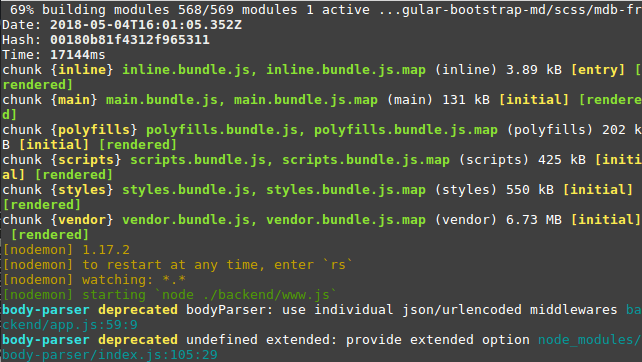
\includegraphics[width=\textwidth]{npm_start_ex}  		
		\caption{Uitvoer van \texttt{npm start} op een linux toestel}
		\label{fig:npm_start_ex}
	\end{figure}
	
	\item Open een nieuwe terminal of console en voer het commando \texttt{ng 
	serve} uit. Dit zal de webapplicatie lokaal starten. Dit commando zal zeggen op 
	welk adres de applicatie draait. Het defaultadres is \texttt{localhost:4200}. 
	Figuur \ref{fig:ng_serve_ex} toont voorbeelduitvoer van dit commando.
	\begin{figure}[ht]
		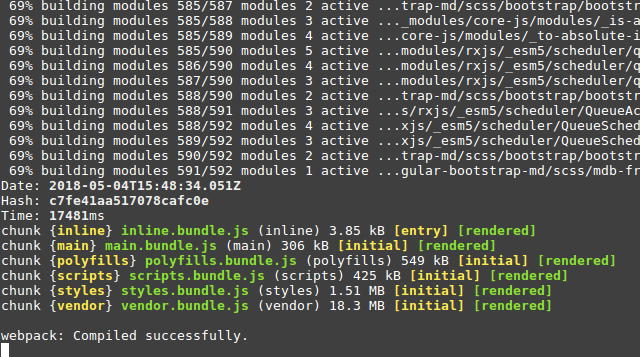
\includegraphics[width=\textwidth]{ng_serve_ex}  
		
		\caption{Uitvoer van \texttt{ng serve} op een linux toestel}
		\label{fig:ng_serve_ex}
	\end{figure}
	
	
	\item Navigeer in een webbrowser naar \texttt{localhost:4200} om de 
	      applicatie te bedienen.
\end{enumerate}



    
\section{Het uitvoeren van testen}
\label{sec:test_exec}
Er zijn twee luiken van testen. Het eerste luik test de operaties die 
worden gebruikt door de webapplicatie. Het tweede luik zijn de JUnit testen voor 
de MP4 Converter.
    
\subsection{Testen van de webapplicatie}
\label{sec:test_exec_web}
De benodigde software is voor dit luik al ge\"installeerd indien de vorige secties correct uitgevoerd zijn. Start de applicatie zoals beschreven in \ref{sec:run_app} en navigeer naar de folder \texttt{annotatietool-01/project} en voer het commando \texttt{npm test} uit. Indien de testen correct zijn uitgevoerd wordt de output van figuur \ref{fig:web_tests} weergegeven.
\begin{figure}[ht]
	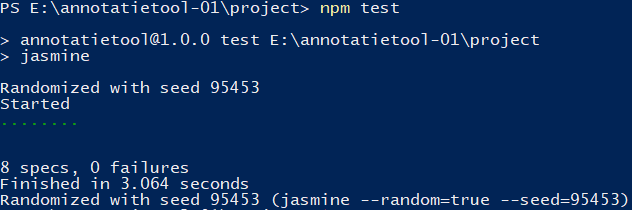
\includegraphics[width=\textwidth]{web_tests}  
	\caption{De uitvoer van correct uitgevoerde integratietesten}
    \label{fig:web_tests}
\end{figure}
\subsection{Testen van de MP4 Converter}
\label{sec:test_exec_java}
Aangezien de MP4 Converter geschreven is in Java is het logisch dat de testsuites geschreven zijn met behulp van JUnit. Indien sectie \ref{sec:hardware_and_software} correct uitgevoerd is, kunnen de JUnit testen uitgevoerd worden. Navigeer vanuit de root folder naar \texttt{java/MP4Converter/} en voer het volgende commando uit:
\texttt{java -jar RunTests.jar}. Om te weten dat alle tests correct uitgevoerd worden zou de output van figuur \ref{fig:java_tests} tevoorschijn moeten komen.
\begin{figure}[ht]
	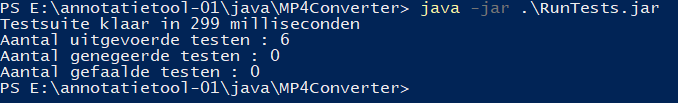
\includegraphics[width=\textwidth]{java_tests}  
	\caption{De uitvoer van correct uitgevoerde JUnit testen}
    \label{fig:java_tests}
\end{figure}

    
\end{document}
